\section{Register Recycling, If-Closure and Address Calculation}
\label{sec:complications}

\subsection{Register Recycling}

The semantics considered thus far assume that each register is assigned at
most once in a program.  We relax this by renaming in the usual way.  Rather
than renaming using arbitrary fresh registers, we use the set
$\uRegs{\AllEvents}=\{\uReg{\aEv}\mid\aEv\in\AllEvents\}$, which are banned
from source programs, as per \textsection\ref{sec:prelim}.  This allows us to
resolve nondeterminism in loads when merging (see
\textsection\ref{sec:redundant}).


\begin{definition}[$\xRecycle$]
  \label{def:pomsets-if}
  Update \refdef{def:pomsets-trans} to:
  \begin{enumerate}
  \item[\ref{L4})] 
    $\aTr{\bEvs}{\bForm}$ implies $\aVal_\aEv{=}\uReg{\aEv}\limplies\bForm[\uReg{\aEv}/\aReg]$, 
  \item[\ref{L5})] 
    $\aTr{\cEvs}{\bForm}$ implies $(\aVal_\aEv{=}\uReg{\aEv}\lor \aLoc{=}\uReg{\aEv})\allowbreak\limplies\bForm[\uReg{\aEv}/\aReg]$,
  \item[\ref{L6})] 
    $(\forall\bReg)$ $\aTr{\dEvs}{\bForm}$ implies $\bForm[\bReg/\aReg]$. 
  \end{enumerate}
\end{definition}

\subsection{If-Closure ($\xIF$)}
\label{sec:if}

% x+0 = x
% if (y==0) { x+y 

% Requires indexing to resolve nondeterminism.

% IF closure/case analysis: $\psi_e$

\begin{example}
  \label{ex:if1}
  \refdef{def:pomsets-trans} does \emph{not} allow:
  \begin{gather*}
    \aCmd=\PBR{
      \PW{x}{0}\SEMI
      \PW{x}{\BANG\BANG r}\SEMI
      \PW{x}{1}
    }
    \\
    \hbox{\begin{tikzinline}[node distance=1em]
        \event{a}{\DW{x}{0}}{}
        \event{b}{\DW{x}{1}}{right=of a}
        \wk{a}{b}
      \end{tikzinline}}
  \end{gather*}
  However, for any $\aForm$, \refdef{def:pomsets-trans} \emph{does} allow:
  \begin{gather*}
    \IF{\aForm}\THEN\aCmd\ELSE\aCmd\FI
    \\
    \hbox{\begin{tikzinline}[node distance=1em]
        \event{a}{\DW{x}{0}}{}
        \event{b}{\DW{x}{1}}{right=of a}
        \wk{a}{b}
      \end{tikzinline}}
  \end{gather*}
  If $r=0$, the middle store can merge left; otherwise, it can merge right.
\end{example}

The difficulty is that any pomset can contain at most one event for the
middle store.  Our solution is to allow a pomset to contain many events for a
single action, as long as the events have disjoint preconditions.

\begin{definition}[$\xRecycle$/$\xIF$]
  \label{def:pomsets-if}
  Update \refdef{def:pomsets-trans} to:

  If $\aPS \in \sSTOREtight[\amode]{\aLoc}{\aExp}$ then
  $(\exists\aVal:\aEvs\fun\Val)$
  $(\exists\cForm:\aEvs\fun\Formulae)$
  \begin{enumerate}
  \item[\ref{S1})] if $\cForm_\bEv\land\cForm_\aEv$ is satisfiable then $\bEv=\aEv$,
  \item[\ref{S2})] $\labelingAct(\aEv) = \DWREFP{\cVal_\aEv}{\aVal_\aEv}$,
  \item[\ref{S3})] $\labelingForm(\aEv)$ implies $\cForm_\aEv \land \aExp{=}\aVal$,
  \item[\ref{S4})] $(\forall\aEv\in\aEvs\cap\bEvs)$
    $\aTr{\bEvs}{\bForm}$ implies $\cForm_\aEv \limplies \bForm[\aExp/\aLoc]$,
  \item[\ref{S5})] 
    $\aTr{\cEvs}{\bForm}$ implies $(\!\not\exists\aEv\in\aEvs\cap\cEvs \suchthat \cForm_\aEv) \limplies \bForm[\aExp/\aLoc]$,
  \end{enumerate}

  If $\aPS \in \sLOAD[\amode]{\aReg}{\aLoc}$ then
  $(\exists\aVal:\aEvs\fun\Val)$
  $(\exists\cForm:\aEvs\fun\Formulae)$
  \begin{enumerate}
  \item[\ref{L1})] if $\cForm_\bEv\land\cForm_\aEv$ is satisfiable then $\bEv=\aEv$,
  \item[\ref{L2})] $\labelingAct(\aEv) = \DRREFP{\cVal_\aEv}{\aVal_\aEv}$,
  \item[\ref{L3})] $\labelingForm(\aEv)$ implies $\cForm_\aEv$.
  \item[\ref{L4})] $(\forall\aEv\in\aEvs\cap\bEvs)$
    $\aTr{\bEvs}{\bForm}$ implies $\cForm_\aEv \limplies \aVal_\aEv{=}\uReg{\aEv}\limplies\bForm[\uReg{\aEv}/\aReg]$, 
  \item[\ref{L5})] $(\forall\aEv\in\aEvs\setminus\cEvs)$
    $\aTr{\cEvs}{\bForm}$ implies $\cForm_\aEv \limplies (\aVal_\aEv{=}\uReg{\aEv}\lor \aLoc{=}\uReg{\aEv})\allowbreak\limplies\bForm[\uReg{\aEv}/\aReg]$,
  \item[\ref{L6})] $(\forall\bReg)$
    $\aTr{\dEvs}{\bForm}$ implies $(\!\not\exists\aEv\in\aEvs \suchthat \cForm_\aEv) \limplies \bForm[\bReg/\aReg]$. 
  \end{enumerate}  
\end{definition}

\begin{example}
  Revisiting \refex{ex:if1}, we can split the middle store:
  \begin{align*}
    \begin{gathered}
      \PW{x}{0}
      \\
      \hbox{\begin{tikzinline}[node distance=.5em and 1.5em]
          \xform{xd}{\bForm[0/x]}{}
          \event{a}{\DW{x}{0}}{above=of xd}      
          \xform{xi}{\bForm[0/x]}{above=of a}
          \xo{a}{xd}
        \end{tikzinline}}
    \end{gathered}
    &&
    \begin{gathered}
      \PW{x}{\BANG\BANG r}
      \\
      \hbox{\begin{tikzinline}[node distance=.5em and 1.5em]
          \xform{xdi}{r{=}0\limplies\bForm[\BANG\BANG r/x]}{}
          \xform{xid}{r{\neq}0\limplies\bForm[\BANG\BANG r/x]}{right=.5em of xdi}
          \event{a}{r{=}0\mid\DW{x}{0}}{above=of xdi}      
          \xo{a}{xdi}
          \event{b}{r{\neq}0\mid\DW{x}{1}}{above=of xid}      
          \xo{b}{xid}
          \xform{xdd}{\bForm[\BANG\BANG r/x]}{above=of a}
          \xform{xii}{\bForm[\BANG\BANG r/x]}{above=of b}
          \xo{a}{xdd}
          \xo{b}{xdd}
        \end{tikzinline}}
    \end{gathered}
    &&
    \begin{gathered}
      \PW{x}{1}
      \\
      \hbox{\begin{tikzinline}[node distance=.5em and 1.5em]
          \xform{xd}{\bForm[1/x]}{}
          \event{a}{\DW{x}{1}}{above=of xd}      
          \xform{xi}{\bForm[1/x]}{above=of a}
          \xo{a}{xd}
        \end{tikzinline}}
    \end{gathered}
  \end{align*}
  Associating to the left and merging, we have:
  \begin{align*}
    \begin{gathered}
      \PW{x}{0}\SEMI
      \PW{x}{\BANG\BANG r}
      \\
      \hbox{\begin{tikzinline}[node distance=.5em and 1.5em]
          \xform{xdi}{r{=}0\limplies\bForm[\BANG\BANG r/x]}{}
          \xform{xid}{r{\neq}0\limplies\bForm[\BANG\BANG r/x]}{right=.5em of xdi}
          \event{a}{\DW{x}{0}}{above=of xdi}      
          \xo{a}{xdi}
          \event{b}{r{\neq}0\mid\DW{x}{1}}{above=of xid}      
          \xo{b}{xid}
          \xform{xdd}{\bForm[\BANG\BANG r/x]}{above=of a}
          \xform{xii}{\bForm[\BANG\BANG r/x]}{above=of b}
          \xo{a}{xdd}
          \xo{b}{xdd}
        \end{tikzinline}}
    \end{gathered}
    &&
    \begin{gathered}
      \PW{x}{1}
      \\
      \hbox{\begin{tikzinline}[node distance=.5em and 1.5em]
          \xform{xd}{\bForm[1/x]}{}
          \event{a}{\DW{x}{1}}{above=of xd}      
          \xform{xi}{\bForm[1/x]}{above=of a}
          \xo{a}{xd}
        \end{tikzinline}}
    \end{gathered}
  \end{align*}
  The merging right, we have, as desired:
  \begin{align*}
    \begin{gathered}
      \PW{x}{0}\SEMI
      \PW{x}{\BANG\BANG r}\SEMI
      \PW{x}{1}
      \\
      \hbox{\begin{tikzinline}[node distance=.5em and 1.5em]
          \xform{xdi}{r{=}0\limplies\bForm[1/x]}{}
          \xform{xid}{r{\neq}0\limplies\bForm[1/x]}{right=of xdi}
          \event{a}{\DW{x}{0}}{above=of xdi}      
          \xo{a}{xdi}
          \event{b}{\DW{x}{1}}{above=of xid}      
          \xo{b}{xid}
          \xform{xdd}{\bForm[1/x]}{above=of a}
          \xform{xii}{\bForm[1/x]}{above=of b}
          \xo{a}{xdd}
          \xo{b}{xdd}
        \end{tikzinline}}
    \end{gathered}
  \end{align*}
\end{example}

\subsection{Address Calculation ($\xADDR$)}

\begin{definition}[$\xADDR$]
  \label{def:pomsets-addr}
  Update \refdef{def:pomsets-trans} to existentially quantify over $\cVal$
  in $\sSTORE{}{}$ and $\sLOAD{}{}$:
  \begin{enumerate}
  \item[\ref{S2})] $\labelingAct(\aEv) = \DW{\REF\cVal}{\aVal}$,
  \item[\ref{L2})] $\labelingAct(\aEv) = \DR{\REF{\cVal}}{\aVal}$.
  \end{enumerate}

  \begin{enumerate}
  \item[\ref{S3})] $\labelingForm(\aEv)$ implies $\cExp{=}\cVal \land \aExp{=}\aVal$,
  \item[\ref{L3})] $\labelingForm(\aEv)$ implies $\cExp{=}\cVal$.
  \end{enumerate}

  \begin{enumerate}
  \item[\ref{S4})] $(\forall\dVal)$ $\aTr{\bEvs}{\bForm}$ implies $\cExp{=}\dVal \limplies \bForm[\aExp/\REF{\dVal}]$,
  \item[\ref{S5})] $(\forall\dVal)$ $\aTr{\cEvs}{\bForm}$ implies $\cExp{=}\dVal \limplies \bForm[\aExp/\REF{\dVal}]$,
  \item[\ref{L4})] $(\forall\dVal)$ $\aTr{\bEvs}{\bForm}$ implies $\cExp{=}\dVal \limplies \aVal{=}\aReg\limplies\bForm$, 
  \item[\ref{L5})] $(\forall\dVal)$ $\aTr{\cEvs}{\bForm}$ implies $\cExp{=}\dVal \limplies (\aVal{=}\aReg\lor \REF{\dVal}{=}\aReg)\limplies\bForm$,
  \item[\ref{L6})] $(\forall\dVal)$ $\aTr{\dEvs}{\bForm}$ implies $\cExp{=}\dVal \limplies \bForm$.
  \end{enumerate}  
\end{definition}

\begin{example}
  punning badly:
  Consider that
  \begin{math}
    \sem{\REF{r} \GETS 0\SEMI \REF{0}\GETS \BANG r}
  \end{math}
  includes both of the following pomsets
  % (``$\BANG$'' is logical
  % negation---``$\BANG \aExp$'' evaluates to $1$ if
  % $\aExp$ is $0$, and $0$ otherwise):
  \begin{align*}
    \begin{gathered}
      \REF{r} \GETS 0\SEMI \REF{0}\GETS \BANG r
      \\
      \hbox{\begin{tikzinline}[node distance=1em]
          \eventl{d}{a}{r\EQ0\mathbin{\mid}\DW{\REF{0}}{0}}{}
          \eventl{e}{b}{r\EQ0\mathbin{\mid}\DW{\REF{0}}{1}}{below=of a}
          \wk{a}{b}
        \end{tikzinline}}
    \end{gathered}
    &&
    \begin{gathered}
      \REF{r} \GETS 0\SEMI \REF{0}\GETS \BANG r
      \\
      \hbox{\begin{tikzinline}[node distance=1em]
          \eventl{c}{a}{r\EQ1\mathbin{\mid}\DW{\REF{1}}{0}}{}
          \eventl{d}{b}{r\EQ1\mathbin{\mid}\DW{\REF{0}}{0}}{below=of a}
        \end{tikzinline}}
    \end{gathered}
  \end{align*}
  Thus, the disjunction closure also includes both of the following: % By using \!$\PAR$\!, it also includes:
  \begin{align*}
    \hbox{\begin{tikzinline}[node distance=1em]
        \eventl{d}{a}{r\EQ0\lor r\EQ1\mathbin{\mid}\DW{\REF{0}}{0}}{}
        \eventl{e}{b}{r\EQ0\mathbin{\mid}\DW{\REF{0}}{1}}{below=of a}
        \wk{a}{b}
      \end{tikzinline}}
    &&
    \hbox{\begin{tikzinline}[node distance=1em]
        \eventl{c}{a}{r\EQ1\mathbin{\mid}\DW{\REF{1}}{0}}{}
        \eventl{d}{b}{r\EQ0\lor r\EQ1\mathbin{\mid}\DW{\REF{0}}{0}}{below=of a}
      \end{tikzinline}}
  \end{align*}
  In this example, the $d$ events that coalesce come from inconsistent executions.
  This is possible because the $d$ events originate from different commands.
\end{example}

% \subsection{Agda}
% \begin{figure*}
%   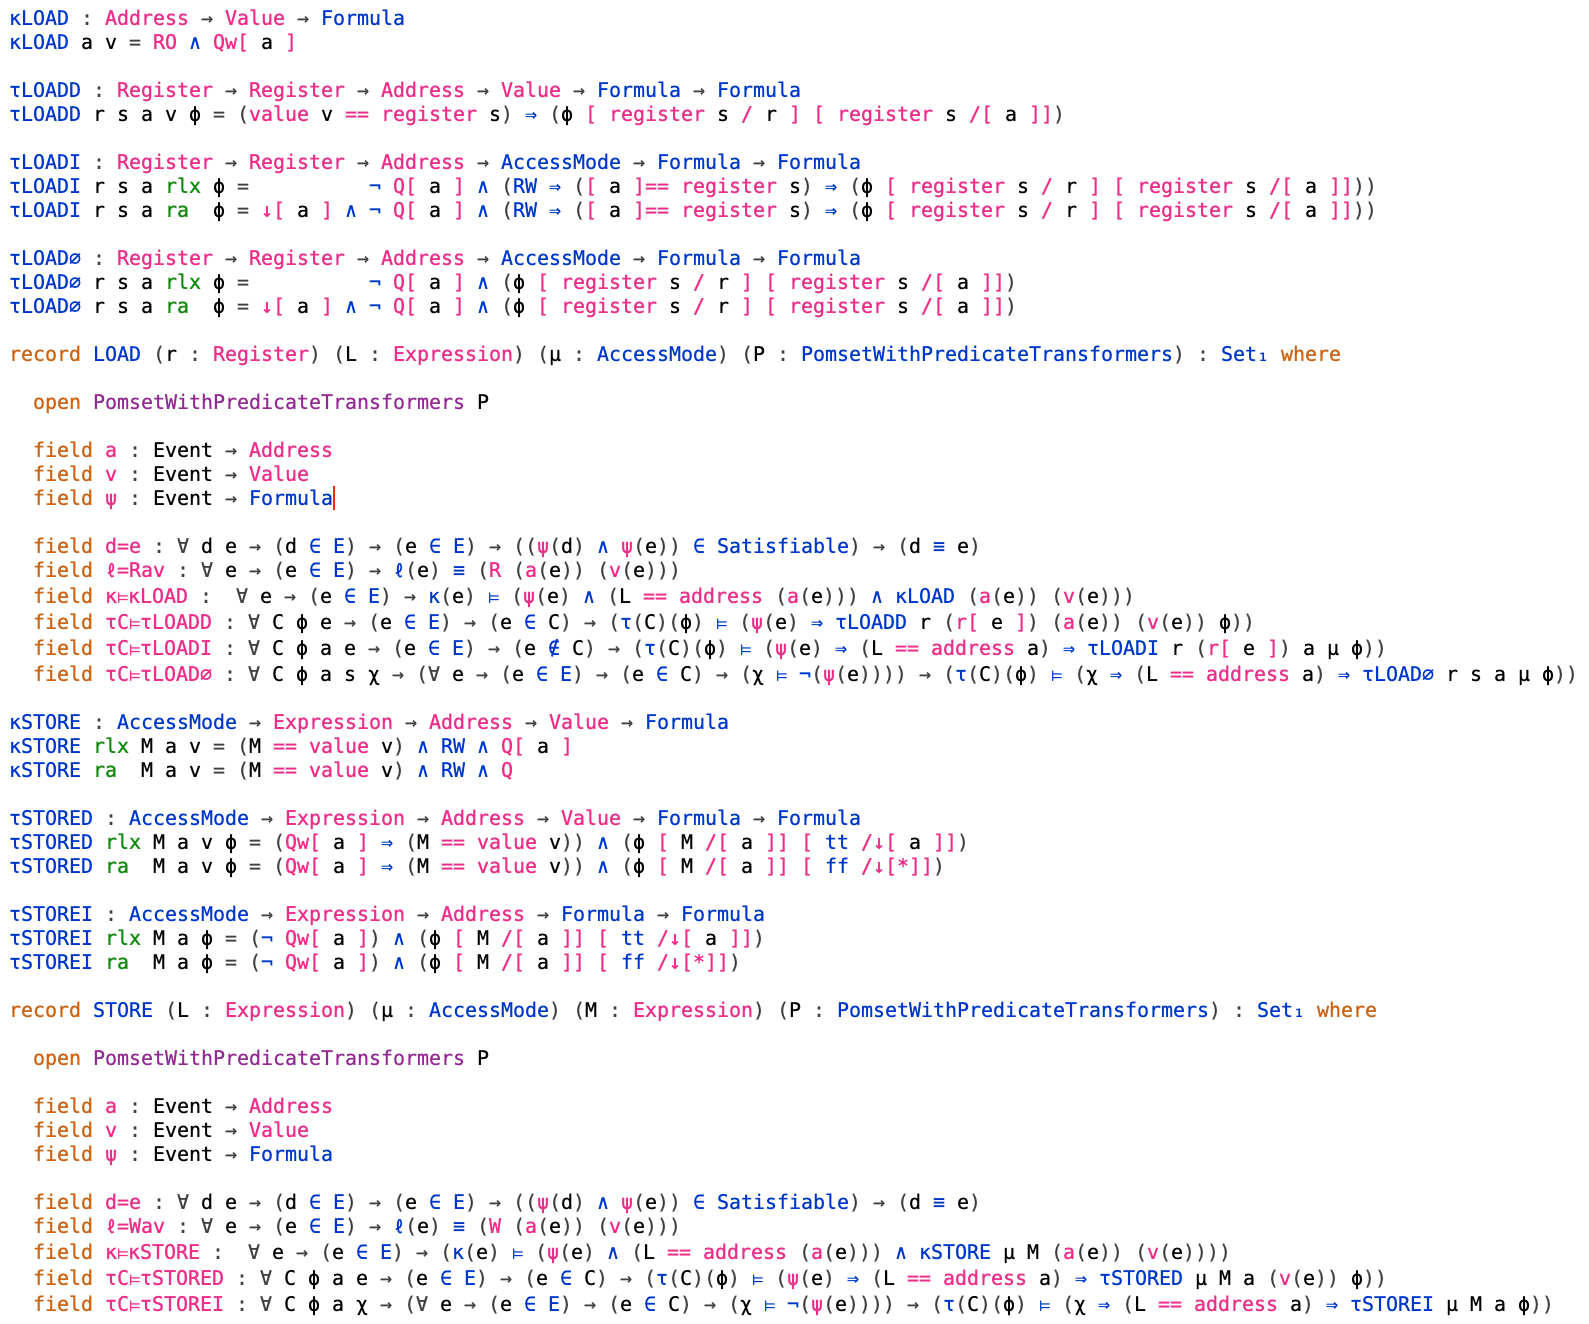
\includegraphics[width=\textwidth]{agda.png}
% \end{figure*}
